% Options for packages loaded elsewhere
\PassOptionsToPackage{unicode}{hyperref}
\PassOptionsToPackage{hyphens}{url}
%
\documentclass[
  english,
  man,floatsintext]{apa6}
\usepackage{lmodern}
\usepackage{amsmath}
\usepackage{ifxetex,ifluatex}
\ifnum 0\ifxetex 1\fi\ifluatex 1\fi=0 % if pdftex
  \usepackage[T1]{fontenc}
  \usepackage[utf8]{inputenc}
  \usepackage{textcomp} % provide euro and other symbols
  \usepackage{amssymb}
\else % if luatex or xetex
  \usepackage{unicode-math}
  \defaultfontfeatures{Scale=MatchLowercase}
  \defaultfontfeatures[\rmfamily]{Ligatures=TeX,Scale=1}
\fi
% Use upquote if available, for straight quotes in verbatim environments
\IfFileExists{upquote.sty}{\usepackage{upquote}}{}
\IfFileExists{microtype.sty}{% use microtype if available
  \usepackage[]{microtype}
  \UseMicrotypeSet[protrusion]{basicmath} % disable protrusion for tt fonts
}{}
\makeatletter
\@ifundefined{KOMAClassName}{% if non-KOMA class
  \IfFileExists{parskip.sty}{%
    \usepackage{parskip}
  }{% else
    \setlength{\parindent}{0pt}
    \setlength{\parskip}{6pt plus 2pt minus 1pt}}
}{% if KOMA class
  \KOMAoptions{parskip=half}}
\makeatother
\usepackage{xcolor}
\IfFileExists{xurl.sty}{\usepackage{xurl}}{} % add URL line breaks if available
\IfFileExists{bookmark.sty}{\usepackage{bookmark}}{\usepackage{hyperref}}
\hypersetup{
  pdftitle={Through the eyes of the teacher},
  pdfauthor={Mandy Klatt1, Dr.~Gregor Kachel1, 2, Dr.~Christin Lotz1, \& Prof.~Dr.~Anne Deiglmayr1},
  pdflang={en-EN},
  pdfkeywords={Professional Vision, Expert-Novice-Paradigm, Eye-Tracking},
  hidelinks,
  pdfcreator={LaTeX via pandoc}}
\urlstyle{same} % disable monospaced font for URLs
\usepackage{graphicx}
\makeatletter
\def\maxwidth{\ifdim\Gin@nat@width>\linewidth\linewidth\else\Gin@nat@width\fi}
\def\maxheight{\ifdim\Gin@nat@height>\textheight\textheight\else\Gin@nat@height\fi}
\makeatother
% Scale images if necessary, so that they will not overflow the page
% margins by default, and it is still possible to overwrite the defaults
% using explicit options in \includegraphics[width, height, ...]{}
\setkeys{Gin}{width=\maxwidth,height=\maxheight,keepaspectratio}
% Set default figure placement to htbp
\makeatletter
\def\fps@figure{htbp}
\makeatother
\setlength{\emergencystretch}{3em} % prevent overfull lines
\providecommand{\tightlist}{%
  \setlength{\itemsep}{0pt}\setlength{\parskip}{0pt}}
\setcounter{secnumdepth}{-\maxdimen} % remove section numbering
% Make \paragraph and \subparagraph free-standing
\ifx\paragraph\undefined\else
  \let\oldparagraph\paragraph
  \renewcommand{\paragraph}[1]{\oldparagraph{#1}\mbox{}}
\fi
\ifx\subparagraph\undefined\else
  \let\oldsubparagraph\subparagraph
  \renewcommand{\subparagraph}[1]{\oldsubparagraph{#1}\mbox{}}
\fi
% Manuscript styling
\usepackage{upgreek}
\captionsetup{font=singlespacing,justification=justified}

% Table formatting
\usepackage{longtable}
\usepackage{lscape}
% \usepackage[counterclockwise]{rotating}   % Landscape page setup for large tables
\usepackage{multirow}		% Table styling
\usepackage{tabularx}		% Control Column width
\usepackage[flushleft]{threeparttable}	% Allows for three part tables with a specified notes section
\usepackage{threeparttablex}            % Lets threeparttable work with longtable

% Create new environments so endfloat can handle them
% \newenvironment{ltable}
%   {\begin{landscape}\begin{center}\begin{threeparttable}}
%   {\end{threeparttable}\end{center}\end{landscape}}
\newenvironment{lltable}{\begin{landscape}\begin{center}\begin{ThreePartTable}}{\end{ThreePartTable}\end{center}\end{landscape}}

% Enables adjusting longtable caption width to table width
% Solution found at http://golatex.de/longtable-mit-caption-so-breit-wie-die-tabelle-t15767.html
\makeatletter
\newcommand\LastLTentrywidth{1em}
\newlength\longtablewidth
\setlength{\longtablewidth}{1in}
\newcommand{\getlongtablewidth}{\begingroup \ifcsname LT@\roman{LT@tables}\endcsname \global\longtablewidth=0pt \renewcommand{\LT@entry}[2]{\global\advance\longtablewidth by ##2\relax\gdef\LastLTentrywidth{##2}}\@nameuse{LT@\roman{LT@tables}} \fi \endgroup}

% \setlength{\parindent}{0.5in}
% \setlength{\parskip}{0pt plus 0pt minus 0pt}

% \usepackage{etoolbox}
\makeatletter
\patchcmd{\HyOrg@maketitle}
  {\section{\normalfont\normalsize\abstractname}}
  {\section*{\normalfont\normalsize\abstractname}}
  {}{\typeout{Failed to patch abstract.}}
\patchcmd{\HyOrg@maketitle}
  {\section{\protect\normalfont{\@title}}}
  {\section*{\protect\normalfont{\@title}}}
  {}{\typeout{Failed to patch title.}}
\makeatother
\shorttitle{Visual attention in teaching and learning processes - QUESTIONNAIRE DATA}
\keywords{Professional Vision, Expert-Novice-Paradigm, Eye-Tracking\newline\indent Word count: 1949}
\usepackage{lineno}

\linenumbers
\usepackage{csquotes}
\ifxetex
  % Load polyglossia as late as possible: uses bidi with RTL langages (e.g. Hebrew, Arabic)
  \usepackage{polyglossia}
  \setmainlanguage[]{english}
\else
  \usepackage[shorthands=off,main=english]{babel}
\fi
\ifluatex
  \usepackage{selnolig}  % disable illegal ligatures
\fi
\newlength{\cslhangindent}
\setlength{\cslhangindent}{1.5em}
\newlength{\csllabelwidth}
\setlength{\csllabelwidth}{3em}
\newenvironment{CSLReferences}[2] % #1 hanging-ident, #2 entry spacing
 {% don't indent paragraphs
  \setlength{\parindent}{0pt}
  % turn on hanging indent if param 1 is 1
  \ifodd #1 \everypar{\setlength{\hangindent}{\cslhangindent}}\ignorespaces\fi
  % set entry spacing
  \ifnum #2 > 0
  \setlength{\parskip}{#2\baselineskip}
  \fi
 }%
 {}
\usepackage{calc}
\newcommand{\CSLBlock}[1]{#1\hfill\break}
\newcommand{\CSLLeftMargin}[1]{\parbox[t]{\csllabelwidth}{#1}}
\newcommand{\CSLRightInline}[1]{\parbox[t]{\linewidth - \csllabelwidth}{#1}\break}
\newcommand{\CSLIndent}[1]{\hspace{\cslhangindent}#1}

\title{Through the eyes of the teacher}
\author{Mandy Klatt\textsuperscript{1}, Dr.~Gregor Kachel\textsuperscript{1, 2}, Dr.~Christin Lotz\textsuperscript{1}, \& Prof.~Dr.~Anne Deiglmayr\textsuperscript{1}}
\date{}


\authornote{

The Ethics Advisory Board of Leipzig University has dealt with the research project and has come to the conclusion that there are no objections to the implementation of this research project. The Ethics Advisory Board points out that the scientific and ethical responsibilty for the implementation of the project remains with the project director.

Correspondence concerning this article should be addressed to Mandy Klatt, Egelstraße 2a 04103 Leipzig. E-mail: \href{mailto:mandy.klatt@uni-leipzig.de}{\nolinkurl{mandy.klatt@uni-leipzig.de}}

}

\affiliation{\vspace{0.5cm}\textsuperscript{1} Leipzig University\\\textsuperscript{2} Max-Planck University for Evolutionary Anthropology}

\abstract{
This document is a supplement to the paper and shows first graphs findings from the pilot study.
}



\begin{document}
\maketitle

\hypertarget{state-of-research}{%
\section{State of research}\label{state-of-research}}

Teaching and classroom management are multidimensional settings in which teachers have to respond immediately to events as they develop (Barnes, 2004). The different interests and abilities of students must be managed in a way that maximizes the active learning time of students and minimizes disruptions whilst teaching. Learning to develop such classroom management skills and to teach effectively is a complicated and complex process (Wolff, Jarodzka, \& Boshuizen, 2017).

During teaching, teachers must be able to select from a variety of visual and acoustic impressions to focus their attention on the essential and to distinguish between relevant and irrelevant events. This ability is called professional vision and is a key component of teacher expertise and successful teaching (Barth, 2017). Eye tracking technology has become a reliable means to study teachers' visual focus of attention (Bogert, 2016; Pouta, Lehtinen, \& Palonen, 2020; Wolff, Jarodzka, \& Boshuizen, 2017)

Educational research has repeatedly shown that there are differences between experienced and novice teachers in terms of perception and behavioral competencies (Barth, 2017; Bogert, 2016; Wolff, Jarodzka, \& Boshuizen, 2017). For example, experts direct their attention more often and more evenly to all students, whereas novices only direct their attention to some students. The frequency and duration of fixations as eye movement are decisive (Stuermer, Seidel, Mueller, Häusler, \& Cortina, 2017). Mobile eye-tracking technology has also shown that experienced teachers distribute their focus more efficiently to solve tasks (Jarodzka, Scheiter, Gerjets, \& Van Gog, 2010). Furthermore, in contrast to novices, experts are able to focus their attention on the entire class and guide the class while giving feedback to individual students and answering questions (Cortina, Miller, McKenzie, \& Epstein, 2015).

\hypertarget{research-questions}{%
\subsection{Research questions}\label{research-questions}}

The aim of the pilot study was to investigate whether there are differences in how expert and novice teachers manage scripted classroom disruptions. The disruptions were experimentally varied using a previously written script. Thus, our aim was to find out whether differences in the allocation of attention between expertise groups can be detected in this controlled context.

In order to answer this question, the hypothesis was formulated that teachers with more professional experience not only notice more disruptions but also notice them faster. In the hypothesis, therefore, it is necessary to check what has already been shown in the research literature: In complex teaching situations, experts have a more structured and elaborate professional knowledge than novices in order to perceive and interpret relevant events and to act appropriately (Berliner, 2001; Lachner, Jarodzka, \& Nückles, 2016).

\hypertarget{methods}{%
\section{Methods}\label{methods}}

We report how we determined our sample size, all data exclusions (if any), all manipulations, and all measures in the study.

\hypertarget{participants}{%
\subsection{Participants}\label{participants}}

For the sample recruitment of the subjects (N = 8, experts n = 2, novices n = 6), schools in the city of Leipzig in Saxony were contacted. The institutions as well as the subjects were informed in detail about the aim and intention of the study in advance. Participation in the study was voluntary and only took place after written consent has been given.

\begin{table}[h]

\begin{center}
\begin{threeparttable}

\caption{\label{tab:demographicspilottable}Demographic Information and Teaching Experience}

\small{

\begin{tabular}{lllllllllll}
\toprule
group & \multicolumn{1}{c}{N} & \multicolumn{1}{c}{Male} & \multicolumn{1}{c}{M age} & \multicolumn{1}{c}{Min age} & \multicolumn{1}{c}{Max age} & \multicolumn{1}{c}{SD age} & \multicolumn{1}{c}{M exp.} & \multicolumn{1}{c}{Min exp.} & \multicolumn{1}{c}{Max exp.} & \multicolumn{1}{c}{SD exp.}\\
\midrule
expert & 2 & 1 & 47.50 & 44 & 51 & 4.95 & 20.00 & 15.00 & 25.00 & 7.07\\
novice & 6 & 2 & 25.67 & 20 & 33 & 4.89 & 0.68 & 0.00 & 1.50 & 0.68\\
\bottomrule
\end{tabular}

}

\end{threeparttable}
\end{center}

\end{table}

The selection of the subjects was based on extreme groups, whereby professional experience is the crucial criterion for the selection of experts or novices. Novices were recruited as teachers who have been working in the teaching profession for no more than 3 years, whereas experts were considered to have professional experience of 10 years or more (Messner \& Reusser, 2000).

\hypertarget{procedure-data-collection}{%
\subsection{Procedure/ Data collection}\label{procedure-data-collection}}

\hypertarget{set-up}{%
\subsubsection{Set up}\label{set-up}}

For this study, scripted mini-lessons with n = 2 experts and n = 6 novices were recorded in the mobile Lab of the Empirical School and Classroom Research at the University of Leipzig. The subjects were divided into groups of four, so the study was conducted on two different sessions. All participants were asked to hold a 10-minute lesson. The duration of each appointment was approximately 2h: per group 10min briefing, 4 x 10min mini-lessons, 10min technical preparation and follow-up and 4x 10min transition points between the lessons and answering questionnaires.

One person from the group of 4 acted as a teacher, the other three subjects acted as the class. The subjects, who represented the class, were given behavioral instructions in a pre-written script to simulate typical events and disruptions in the classroom (e.g.~putting their heads on the table, chatting, looking at their mobile phones, etc.).

The lesson disruptions were displayed as instructions during the lesson for all ``students'' but not the teacher. In order to avoid learning effects, the disruptions in each lesson were distributed pseudo-randomly over the short teaching phase. In addition, the order of the data collection was taken into account in the analyses and variance caused by order was controlled.



\begin{figure}

{\centering 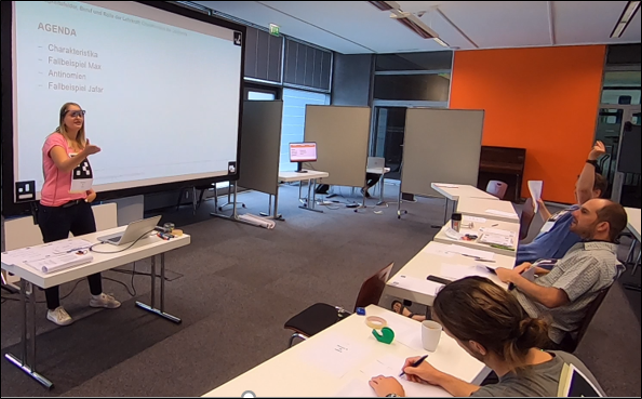
\includegraphics[width=5.94in]{./pictures/datacollection} 

}

\caption{Example for set up during a mini-lesson}\label{fig:datacollection}
\end{figure}

\hypertarget{questionnaire-data}{%
\subsubsection{Questionnaire data}\label{questionnaire-data}}

After each mini-lesson, the students answered items on the teaching quality using a validated questionnaire (Helmke et al., 2014) and scales on the teacher's presence behavior (students n = 24). In addition, the teacher was asked to give a self-assessment on his/her classroom management by completing the questionnaire after each mini-lesson (teachers n = 8).

\hypertarget{coding-data-preparation-reliability}{%
\subsection{Coding/ Data preparation/ Reliability}\label{coding-data-preparation-reliability}}

\hypertarget{questionnaire-data-1}{%
\subsubsection{Questionnaire Data}\label{questionnaire-data-1}}

The evaluation after each mini-lesson was conducted using paper questionnaires. Time needed to complete the questionnaire was about 5 minutes.
The scales on the quality of teaching are a validated questionnaire (Helmke et al., 2014). Whereas the scales on the teacher's presence behavior were derived from the research literature (Brophy, 1986; Kiel, Frey, Weiß, \& Weiss, 2013; Kounin, 2006; Marzano, 2007; Nolting, 2012) and were used in the pilot for the first time. The questionnaire is 4-point Likert scale (1 = Strongly Disagree; 2 = Disagree; 3 = Agree; 4 = Strongly Agree). Data was obtained from N = 32 subjects (students n = 24, teachers n = 8).

The following scales were assessed:

\begin{enumerate}
\def\labelenumi{(\arabic{enumi})}
\tightlist
\item
  Classroom management
\item
  Positive climate and motivation
\item
  Clarity and structuredness
\item
  Activation and support
\item
  Presence: posture/gaze
\item
  Presence: voice
\item
  Presence: verbal and non-verbal intervention
\item
  Natural behaviour
\end{enumerate}

Table \ref{tab:table-all-scales-self-assessment} provides an overview over the mean, the standard deviation, the range, Cronbach's Alpha and the Skewness \& Kurtosis of all scales for the teachers' self-assessment.

\begin{verbatim}
## Some items ( ks_sichtbar ) were negatively correlated with the total scale and 
## probably should be reversed.  
## To do this, run the function again with the 'check.keys=TRUE' option
\end{verbatim}

\begin{verbatim}
## Some items ( pi_nonverbal ) were negatively correlated with the total scale and 
## probably should be reversed.  
## To do this, run the function again with the 'check.keys=TRUE' option
\end{verbatim}

\begin{verbatim}
## Some items ( pi_nonverbal ) were negatively correlated with the total scale and 
## probably should be reversed.  
## To do this, run the function again with the 'check.keys=TRUE' option
\end{verbatim}

\begin{table}[h]

\begin{center}
\begin{threeparttable}

\caption{\label{tab:table-all-scales-self-assessment}Scale analysis for teachers' self-assessment}

\tiny{

\begin{tabular}{lllllllll}
\toprule
scale & \multicolumn{1}{c}{N items} & \multicolumn{1}{c}{M} & \multicolumn{1}{c}{SD} & \multicolumn{1}{c}{Min} & \multicolumn{1}{c}{Max} & \multicolumn{1}{c}{Skewness} & \multicolumn{1}{c}{Kurtosis} & \multicolumn{1}{c}{Cronbach's a}\\
\midrule
Activation and support & 3 & 2.46 & 1.14 & 1 & 4 & 0.10 & 1.65 & 0.85\\
Clarity and structuredness & 2 & 2.81 & 0.91 & 1 & 4 & -0.17 & 2.17 & -0.76\\
Classroom management & 4 & 2.44 & 0.88 & 1 & 4 & 0.19 & 2.38 & 0.83\\
Natural behaviour & 3 & 2.83 & 0.76 & 2 & 4 & 0.28 & 1.84 & 0.90\\
Positive climate and motivation & 6 & 2.85 & 0.87 & 1 & 4 & -0.49 & 2.65 & 0.78\\
Presence: posture/gaze & 7 & 2.70 & 1.01 & 1 & 4 & -0.44 & 2.15 & 0.85\\
Presence: verbal and non-verbal intervention & 3 & 2.75 & 0.79 & 1 & 4 & -0.07 & 2.48 & -0.75\\
Presence: voice & 3 & 2.79 & 0.72 & 2 & 4 & 0.32 & 2.03 & 0.77\\
\bottomrule
\end{tabular}

}

\end{threeparttable}
\end{center}

\end{table}

Table \ref{tab:table-all-scales-students} provides an overview over the mean, the standard deviation, the range, Cronbach's Alpha and the Skewness \& Kurtosis of all scales for the students' perception of the teacher's behaviour in class.

\begin{verbatim}
## Some items ( phb_stand ) were negatively correlated with the total scale and 
## probably should be reversed.  
## To do this, run the function again with the 'check.keys=TRUE' option
\end{verbatim}

\begin{verbatim}
## Some items ( pi_direkt ) were negatively correlated with the total scale and 
## probably should be reversed.  
## To do this, run the function again with the 'check.keys=TRUE' option
\end{verbatim}

\begin{verbatim}
## Some items ( phb_stand ) were negatively correlated with the total scale and 
## probably should be reversed.  
## To do this, run the function again with the 'check.keys=TRUE' option
\end{verbatim}

\begin{table}[h]

\begin{center}
\begin{threeparttable}

\caption{\label{tab:table-all-scales-students}Scale analysis for students' perspective}

\tiny{

\begin{tabular}{lllllllll}
\toprule
scale & \multicolumn{1}{c}{N items} & \multicolumn{1}{c}{M} & \multicolumn{1}{c}{SD} & \multicolumn{1}{c}{Min} & \multicolumn{1}{c}{Max} & \multicolumn{1}{c}{Skewness} & \multicolumn{1}{c}{Kurtosis} & \multicolumn{1}{c}{Cronbach's a}\\
\midrule
Activation and support & 3 & 2.64 & 1.13 & 1 & 4 & -0.32 & 1.73 & 0.48\\
Clarity and structuredness & 2 & 3.58 & 0.68 & 1 & 4 & -1.75 & 6.09 & 0.62\\
Classroom management & 4 & 3.18 & 0.91 & 1 & 4 & -0.87 & 2.86 & 0.75\\
Natural behaviour & 3 & 3.43 & 0.67 & 2 & 4 & -0.74 & 2.46 & 0.85\\
Positive climate and motivation & 6 & 3.41 & 0.83 & 1 & 4 & -1.40 & 4.29 & 0.82\\
Presence: posture/gaze & 7 & 3.24 & 0.89 & 1 & 4 & -1.05 & 3.31 & 0.59\\
Presence: verbal and non-verbal intervention & 3 & 3.18 & 0.81 & 1 & 4 & -0.66 & 2.70 & 0.20\\
Presence: voice & 3 & 3.60 & 0.60 & 2 & 4 & -1.18 & 3.36 & 0.71\\
\bottomrule
\end{tabular}

}

\end{threeparttable}
\end{center}

\end{table}
\newpage

The individual items of a scale are further represented in graphs.

\begin{enumerate}
\def\labelenumi{(\arabic{enumi})}
\item
  Classroom management
  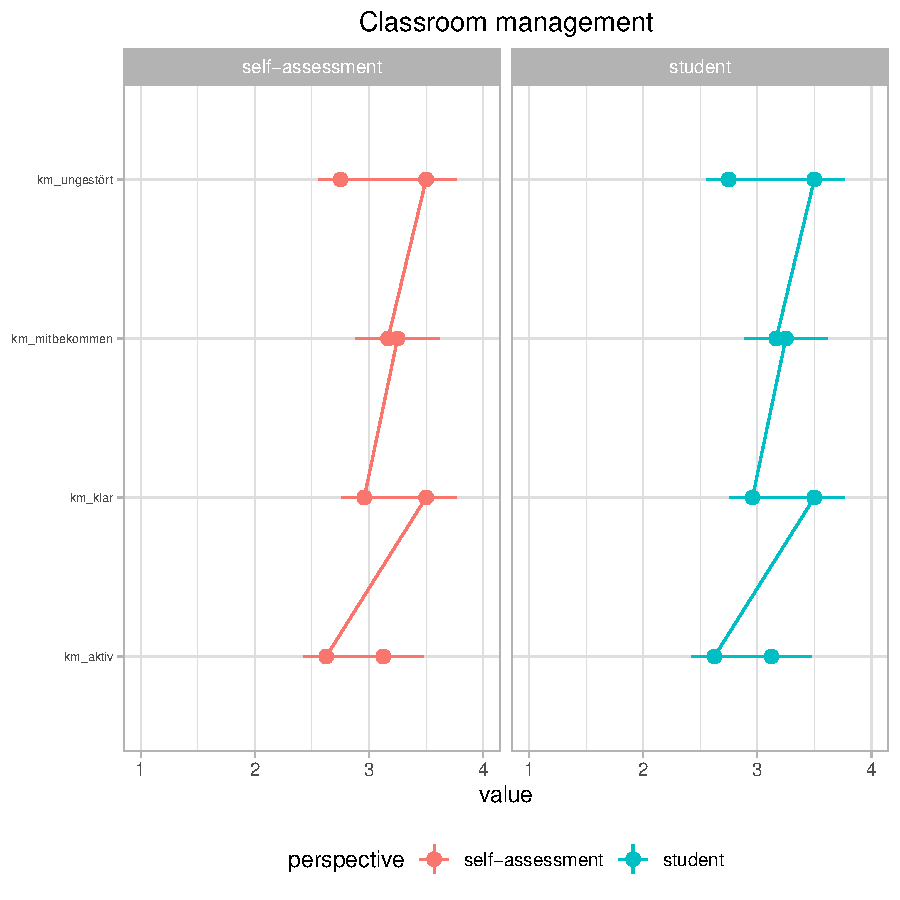
\includegraphics{paper_1_supplement_questionnaire_files/figure-latex/Line Plots Classroom Management-1.pdf}
  \newpage
\item
  Positive climate and motivation
  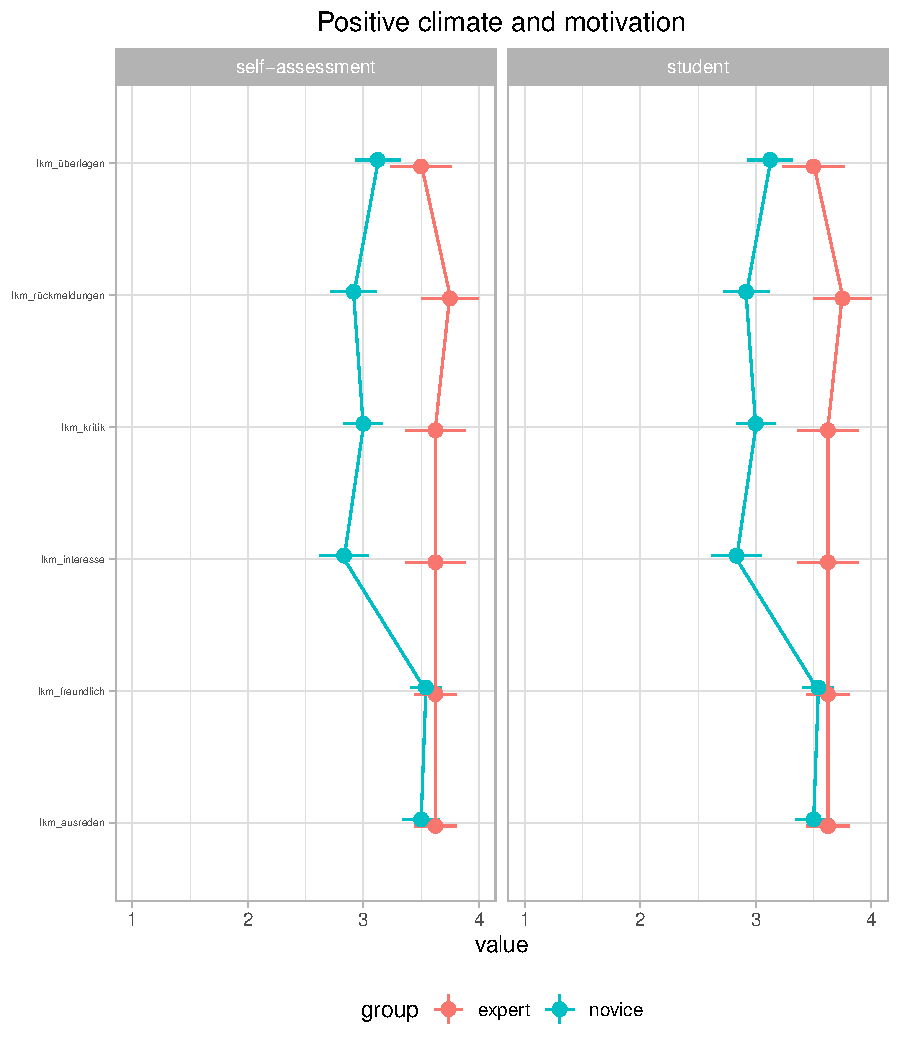
\includegraphics{paper_1_supplement_questionnaire_files/figure-latex/Positive climate and motivation line plots-1.pdf}
  \newpage
\item
  Clarity and structuredness
  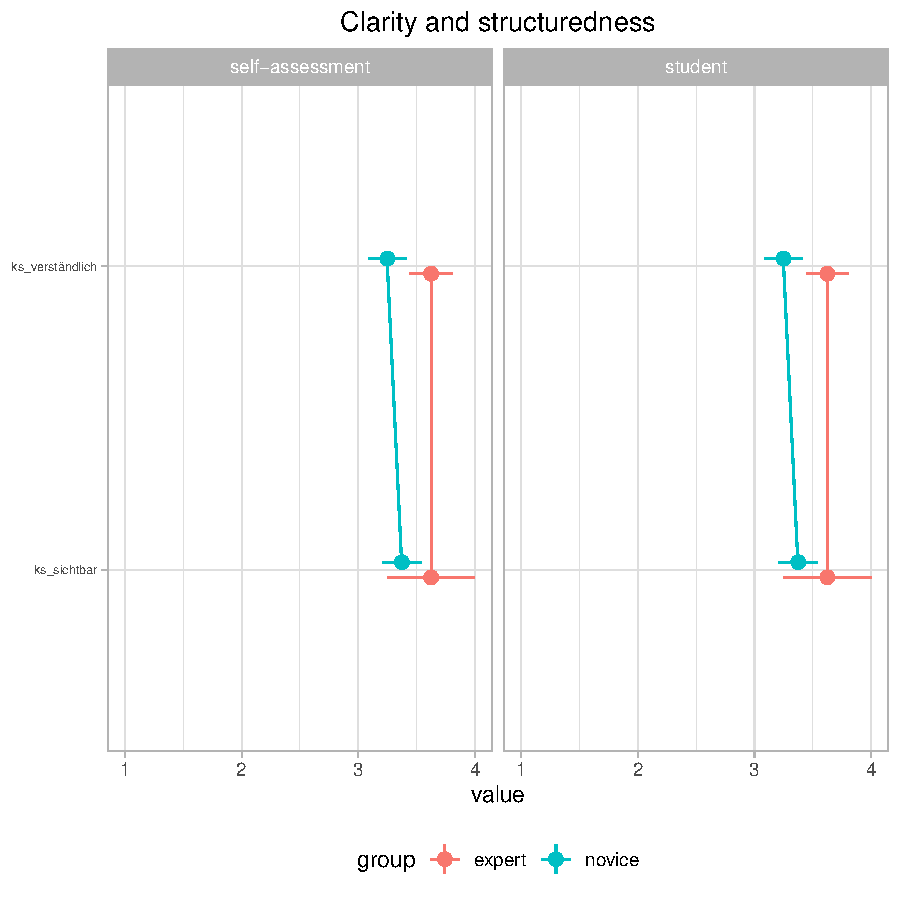
\includegraphics{paper_1_supplement_questionnaire_files/figure-latex/Clarity and structuredness line plots-1.pdf}
  \newpage
\item
  Activation and support
  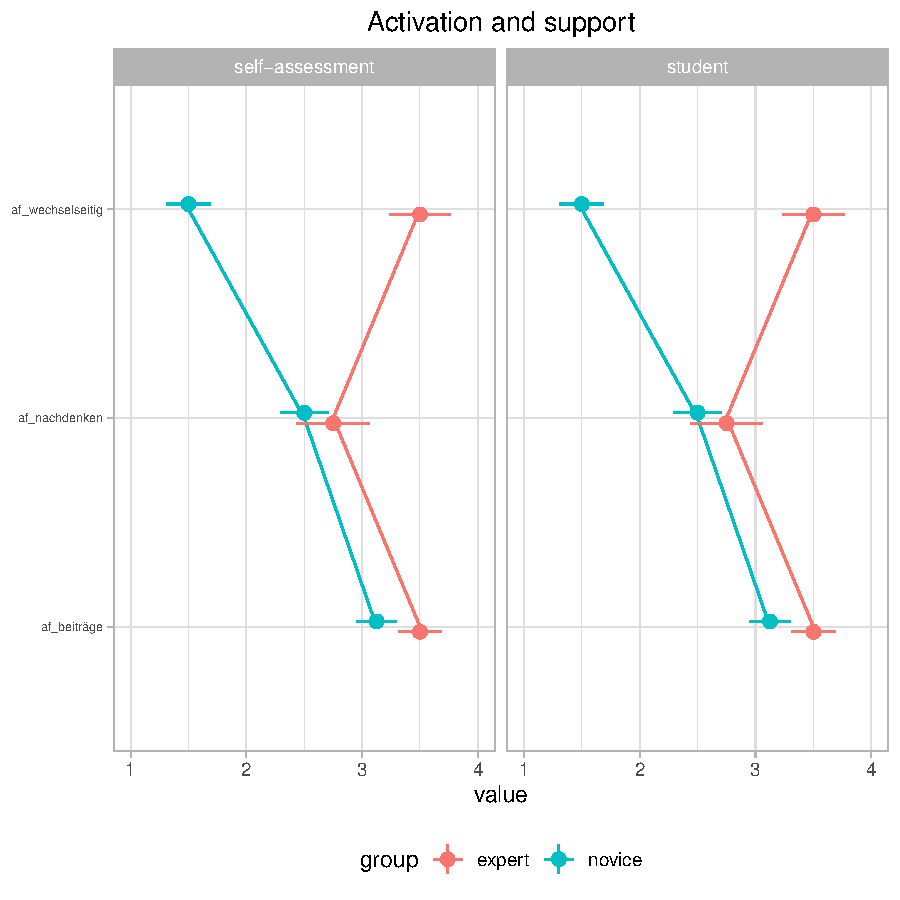
\includegraphics{paper_1_supplement_questionnaire_files/figure-latex/Activation and support line plots-1.pdf}
  \newpage
\item
  Presence: posture and gaze
  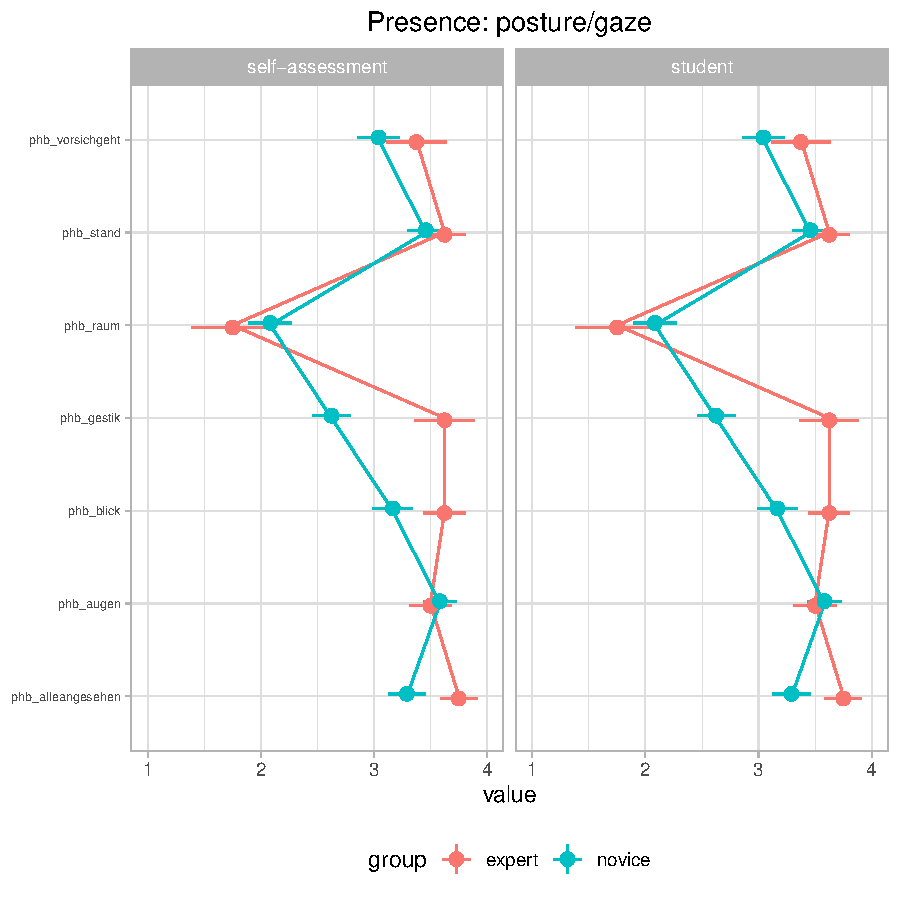
\includegraphics{paper_1_supplement_questionnaire_files/figure-latex/Presence posture and gaze line plots-1.pdf}
\end{enumerate}

\newpage

\begin{enumerate}
\def\labelenumi{(\arabic{enumi})}
\setcounter{enumi}{5}
\item
  Presence: voice
  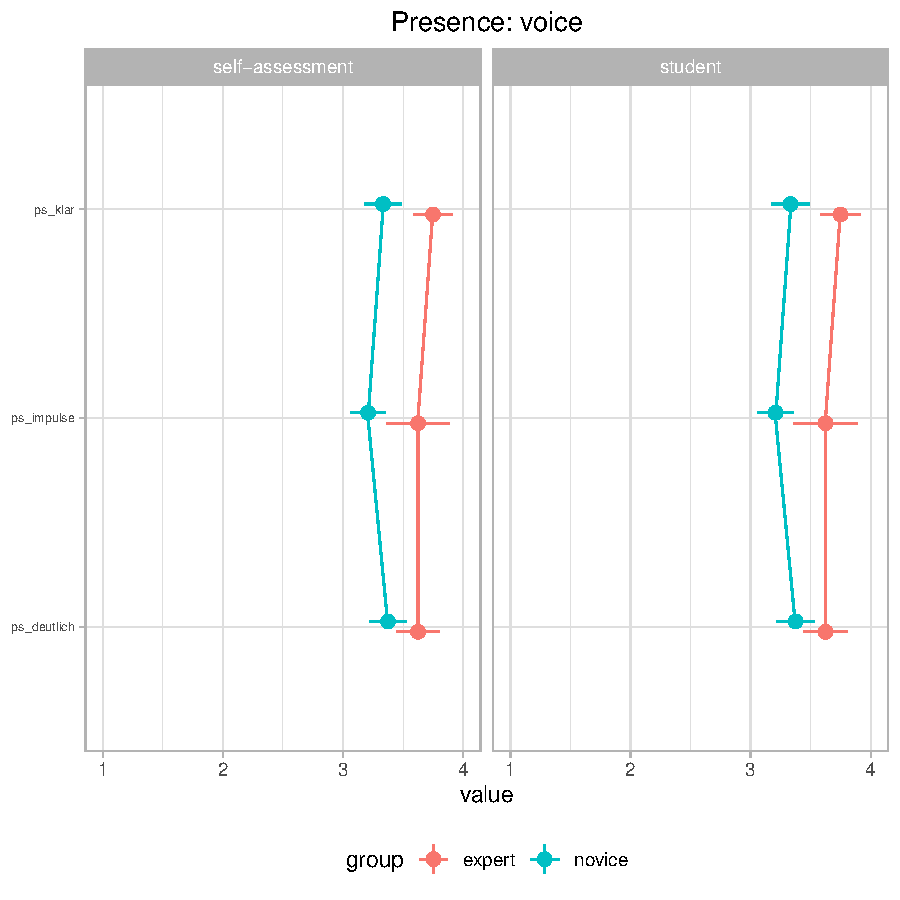
\includegraphics{paper_1_supplement_questionnaire_files/figure-latex/Presence voice line plots-1.pdf}
  \newpage
\item
  Presence: verbal and non-verbal intervention
\end{enumerate}

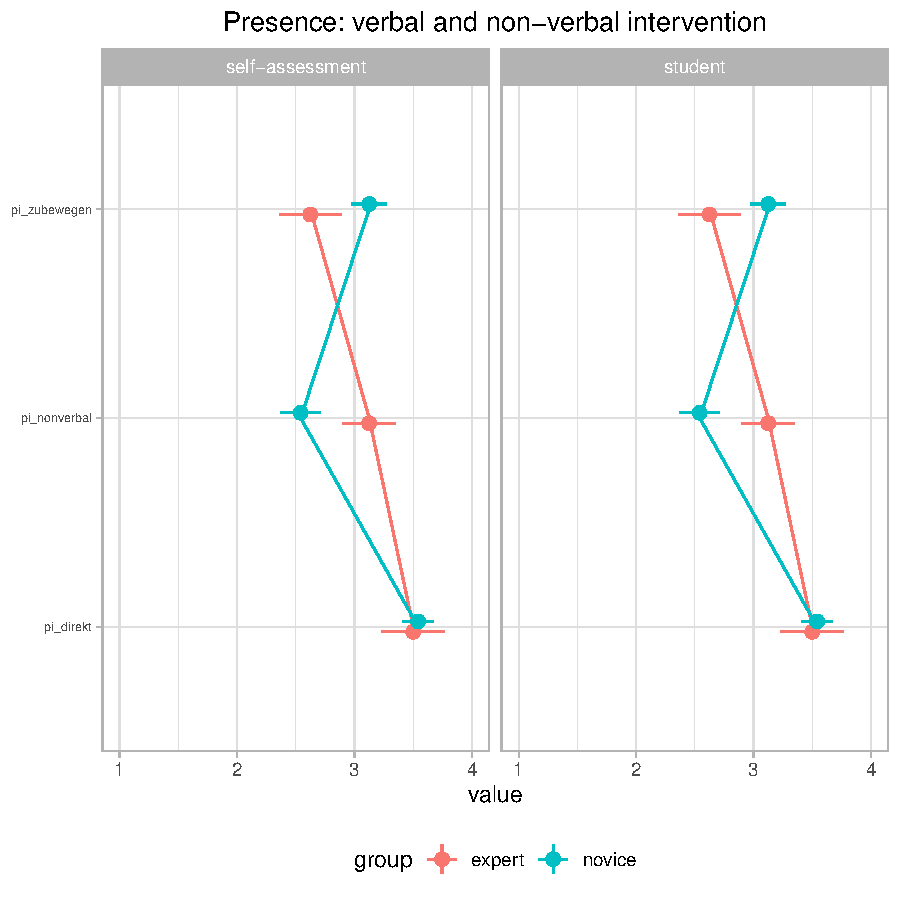
\includegraphics{paper_1_supplement_questionnaire_files/figure-latex/Presence verbal and non-verbal intervention line plots-1.pdf}
\newpage
(8) Natural behaviour
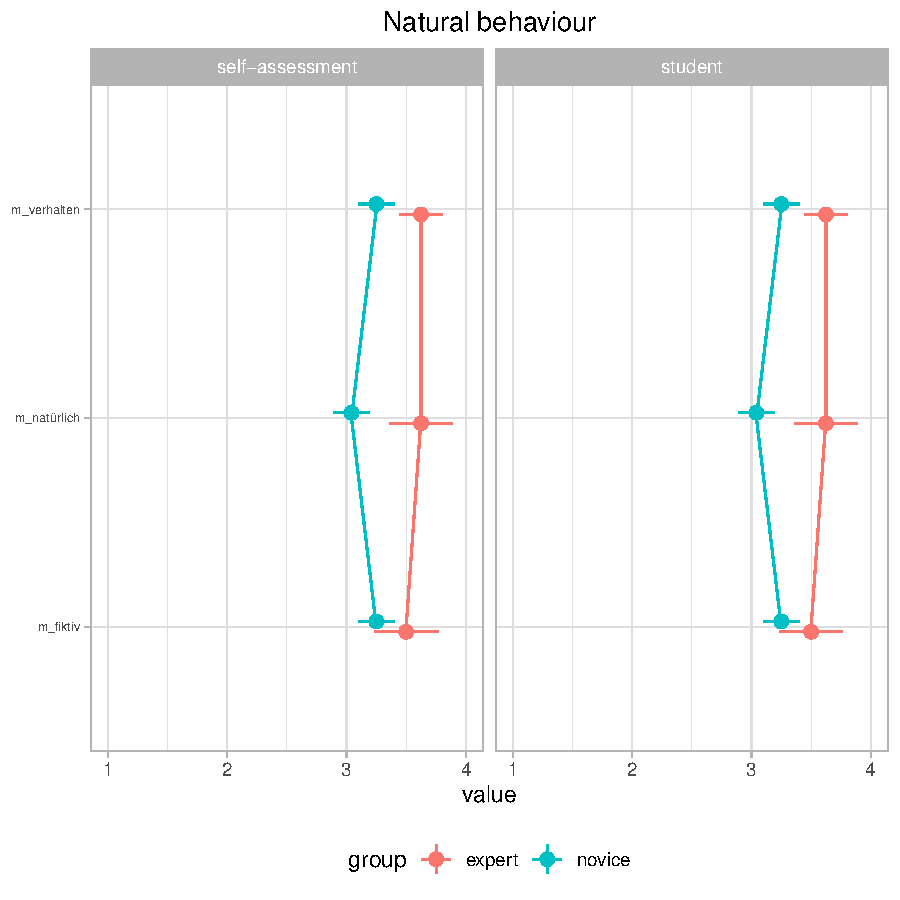
\includegraphics{paper_1_supplement_questionnaire_files/figure-latex/Natural behaviour line plots-1.pdf}
\newpage
In addition, we plotted all scales. Graph provides boxplots and individual data for experts and novices.

\begin{verbatim}
## Warning: Removed 1 rows containing non-finite values (stat_boxplot).
\end{verbatim}

\begin{verbatim}
## Warning: Removed 1 rows containing missing values (geom_point).
\end{verbatim}

\begin{figure}
\centering
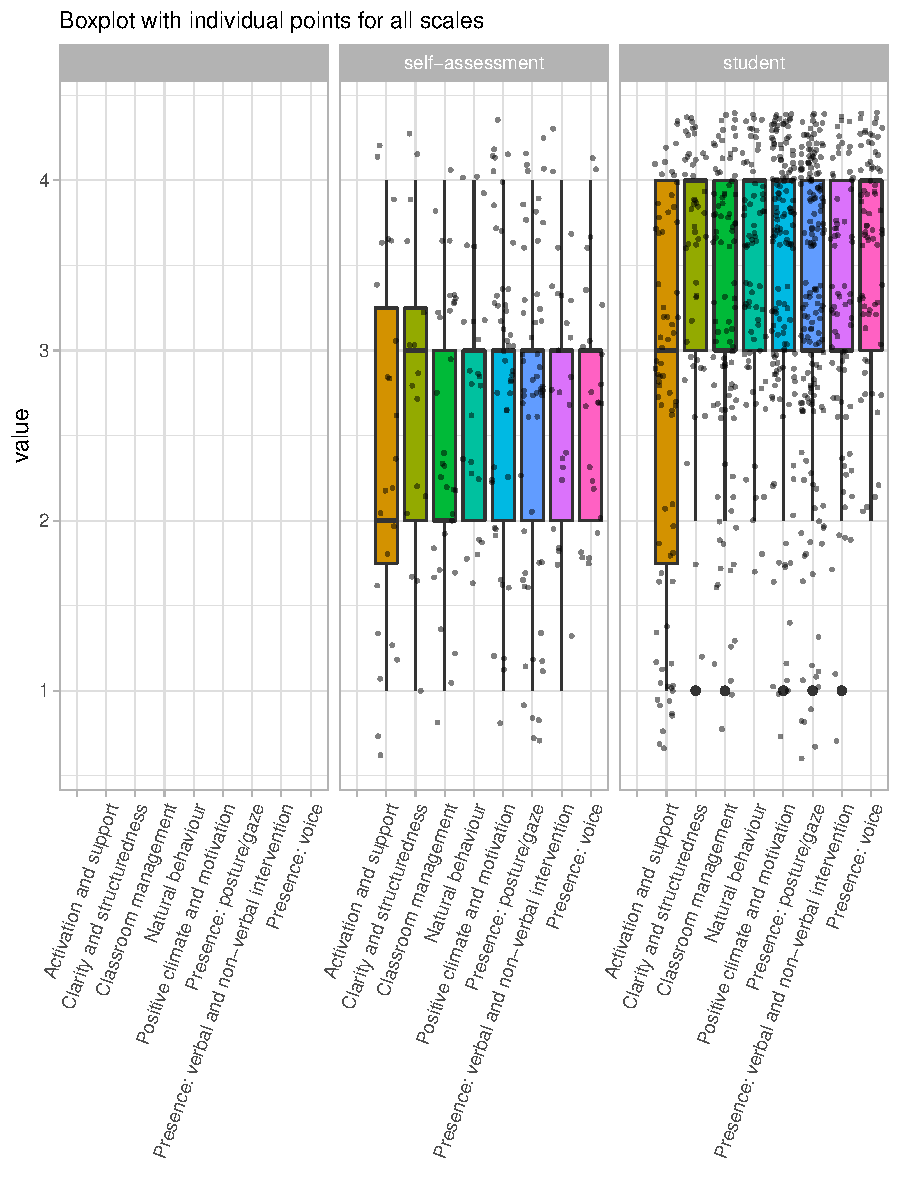
\includegraphics{paper_1_supplement_questionnaire_files/figure-latex/boxplot scales-1.pdf}
\caption{(\#fig:boxplot scales)Boxplots and individual data for experts and novices}
\end{figure}

\hypertarget{refs}{}
\begin{CSLReferences}{1}{0}
\leavevmode\hypertarget{ref-barnes2004significance}{}%
Barnes, D. (2004). The significance of teachers' frames for teaching. In \emph{Teachers and teaching} (pp. 16--38). Routledge.

\leavevmode\hypertarget{ref-barth2017professionelle}{}%
Barth, V. L. (2017). \emph{Professionelle wahrnehmung von störungen im unterricht}. Springer.

\leavevmode\hypertarget{ref-berliner2001learning}{}%
Berliner, D. C. (2001). Learning about and learning from expert teachers. \emph{International Journal of Educational Research}, \emph{35}(5), 463--482.

\leavevmode\hypertarget{ref-bogert2016visualperception}{}%
Bogert, N. J. van den. (2016). \emph{On teachers' visual perception and interpretation of classroom events using eye tracking and collaborative tagging methodologies}. Technische Universiteit Eindhoven.

\leavevmode\hypertarget{ref-brophy1986classroom}{}%
Brophy, J. (1986). Classroom management techniques. \emph{Education and Urban Society}, \emph{18}(2), 182--194.

\leavevmode\hypertarget{ref-cortina2015low}{}%
Cortina, K. S., Miller, K. F., McKenzie, R., \& Epstein, A. (2015). Where low and high inference data converge: Validation of CLASS assessment of mathematics instruction using mobile eye tracking with expert and novice teachers. \emph{International Journal of Science and Mathematics Education}, \emph{13}(2), 389--403.

\leavevmode\hypertarget{ref-helmke2014unterrichtsdiagnostik}{}%
Helmke, A., Helmke, T., Lenske, G., Pham, G., Praetorius, A.-K., Schrader, F.-W., \& AdeThurow, M. (2014). Unterrichtsdiagnostik mit EMU. \emph{Aus-Und Fortbildung Der Lehrkr{ä}fte in Hinblick Auf Verbesserung Der Diagnosef{ä}higkeit, Umgang Mit Heterogenit{ä}t Und Individuelle F{ö}rderung}, 149--163.

\leavevmode\hypertarget{ref-jarodzka2010eyes}{}%
Jarodzka, H., Scheiter, K., Gerjets, P., \& Van Gog, T. (2010). In the eyes of the beholder: How experts and novices interpret dynamic stimuli. \emph{Learning and Instruction}, \emph{20}(2), 146--154.

\leavevmode\hypertarget{ref-kiel2013trainingsbuch}{}%
Kiel, E., Frey, A., Weiß, S., \& Weiss, S. (2013). \emph{Trainingsbuch klassenf{ü}hrung} (Vol. 3992). UTB.

\leavevmode\hypertarget{ref-kounin2006techniken}{}%
Kounin, J. S. (2006). \emph{Techniken der klassenf{ü}hrung}. Waxmann Verlag.

\leavevmode\hypertarget{ref-lachner2016makes}{}%
Lachner, A., Jarodzka, H., \& Nückles, M. (2016). What makes an expert teacher? Investigating teachers' professional vision and discourse abilities. \emph{Instructional Science}, \emph{44}(3), 197--203.

\leavevmode\hypertarget{ref-marzano2007art}{}%
Marzano, R. J. (2007). \emph{The art and science of teaching: A comprehensive framework for effective instruction}. Ascd.

\leavevmode\hypertarget{ref-messner2000berufliche}{}%
Messner, H., \& Reusser, K. (2000). Die berufliche entwicklung von lehrpersonen als lebenslanger prozess. \emph{Beitr{ä}ge Zur Lehrerinnen-Und Lehrerbildung}, \emph{18}(2), 157--171.

\leavevmode\hypertarget{ref-nolting2012storungen}{}%
Nolting, H.-P. (2012). \emph{St{ö}rungen in der schulklasse}. Beltz.

\leavevmode\hypertarget{ref-pouta2020student}{}%
Pouta, M., Lehtinen, E., \& Palonen, T. (2020). Student teachers' and experienced teachers' professional vision of students' understanding of the rational number concept.

\leavevmode\hypertarget{ref-stuermer2017eye}{}%
Stuermer, K., Seidel, T., Mueller, K., Häusler, J., \& Cortina, K. S. (2017). What is in the eye of preservice teachers while instructing? An eye-tracking study about attention processes in different teaching situations. \emph{Zeitschrift f{ü}r Erziehungswissenschaft}, \emph{20}(1), 75--92.

\leavevmode\hypertarget{ref-wolff2017see}{}%
Wolff, C. E., Jarodzka, H., \& Boshuizen, H. P. (2017). See and tell: Differences between expert and novice teachers' interpretations of problematic classroom management events. \emph{Teaching and Teacher Education}, \emph{66}, 295--308.

\end{CSLReferences}


\end{document}
